%%
%% This is file `tikzposter-template.tex',
%% generated with the docstrip utility.
%%
%% The original source files were:
%%
%% tikzposter.dtx  (with options: `tikzposter-template.tex')
%%
%% This is a generated file.
%%
%% Copyright (C) 2014 by Pascal Richter, Elena Botoeva, Richard Barnard, and Dirk Surmann
%%
%% This file may be distributed and/or modified under the
%% conditions of the LaTeX Project Public License, either
%% version 2.0 of this license or (at your option) any later
%% version. The latest version of this license is in:
%%
%% http://www.latex-project.org/lppl.txt
%%
%% and version 2.0 or later is part of all distributions of
%% LaTeX version 2013/12/01 or later.
%%


\documentclass{tikzposter} %Options for format can be included here

\usepackage{todonotes}

\usepackage[tikz]{bclogo}
\usepackage{lipsum}
\usepackage{amsmath}

\usepackage{booktabs}
\usepackage{longtable}
\usepackage[absolute]{textpos}
\usepackage[it]{subfigure}
\usepackage{graphicx}
\usepackage{cmbright}
%\usepackage[default]{cantarell}
%\usepackage{avant}
%\usepackage[math]{iwona}
\usepackage[math]{kurier}
\usepackage[T1]{fontenc}


%% add your packages here
\usepackage{hyperref}
% for random text
\usepackage{lipsum}
\usepackage[english]{babel}
\usepackage[pangram]{blindtext}

\colorlet{backgroundcolor}{blue!10}

 % Title, Author, Institute
\title{FLIP00 FINAL PRESENTATION}
\author{Zhaoyang Wang}
\institute{Xi'an Shiyou University, China
}
%\titlegraphic{logos/tulip-logo.eps}

%Choose Layout
\usetheme{Wave}

%\definebackgroundstyle{samplebackgroundstyle}{
%\draw[inner sep=0pt, line width=0pt, color=red, fill=backgroundcolor!30!black]
%(bottomleft) rectangle (topright);
%}
%
%\colorlet{backgroundcolor}{blue!10}

\begin{document}


\colorlet{blocktitlebgcolor}{blue!23}

 % Title block with title, author, logo, etc.
\maketitle

\begin{columns}
 % FIRST column
\column{0.5}% Width set relative to text width

%%%%%%%%%% -------------------------------------------------------------------- %%%%%%%%%%
 %\block{Main Objectives}{
%  	      	\begin{enumerate}
%  	      	\item Formalise research problem by extending \emph{outlying aspects mining}
%  	      	\item Proposed \emph{GOAM} algorithm is to solve research problem
%  	      	\item Utilise pruning strategies to reduce time complexity
%  	      	\end{enumerate}
%%  	      \end{minipage}
%}
%%%%%%%%%% -------------------------------------------------------------------- %%%%%%%%%%


%%%%%%%%%% -------------------------------------------------------------------- %%%%%%%%%%
\block{Introduction}{
You are given 5 years of store-item sales data, and asked to predict 3 months of sales for 50 different items at 10 different stores.
\vspace{1cm}
\begin{description}
  \item [date] - Date of the sale data. There are no holiday effects or store closures.
  \item [store] - Store ID
  \item [item] - Item ID
  \item [sales] - Number of items sold at a particular store on a particular date.
\end{description}
}
%%%%%%%%%% -------------------------------------------------------------------- %%%%%%%%%%


%%%%%%%%%% -------------------------------------------------------------------- %%%%%%%%%%
\block{Data Visualization}{
By using matplotlib to describe the data.And Observe the relationship between different features.
\vspace{1cm}
\begin{center}
  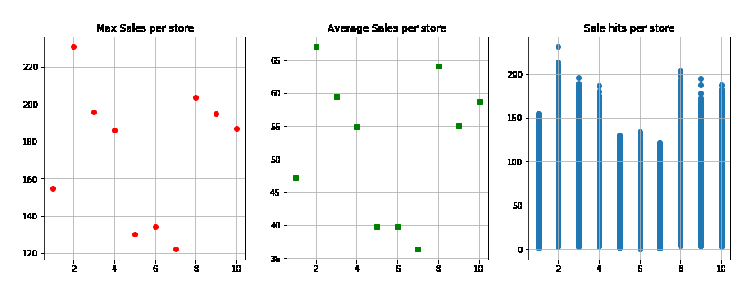
\includegraphics[width=.5\linewidth]{E:/tulip-flip/templatex-master/powerdot-tuliplab/logos/0003.eps}
  \quad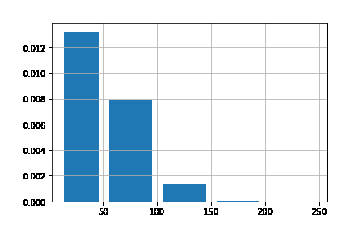
\includegraphics[width=.3\linewidth]{E:/tulip-flip/templatex-master/powerdot-tuliplab/logos/0004.eps}
  \quad\includegraphics[width=.3\linewidth,height=.2\linewidth]{E:/tulip-flip/templatex-master/powerdot-tuliplab/logos/0006.eps}	
  \quad\includegraphics[width=.3\linewidth,height=.2\linewidth]{E:/tulip-flip/templatex-master/powerdot-tuliplab/logos/0007.eps}
  \quad\includegraphics[width=.3\linewidth,height=.2\linewidth]{E:/tulip-flip/templatex-master/powerdot-tuliplab/logos/0008.eps}
  \quad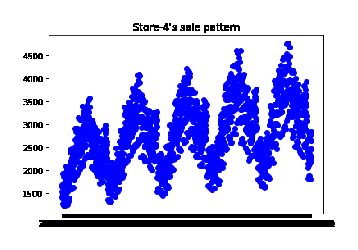
\includegraphics[width=.3\linewidth,height=.25\linewidth]{E:/tulip-flip/templatex-master/powerdot-tuliplab/logos/0009.eps}
  \quad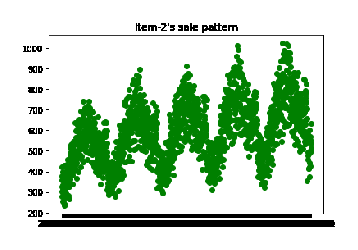
\includegraphics[width=.3\linewidth,height=.25\linewidth]{E:/tulip-flip/templatex-master/powerdot-tuliplab/logos/0010.eps}
\end{center}
}
%%%%%%%%%% -------------------------------------------------------------------- %%%%%%%%%%


%%%%%%%%%% -------------------------------------------------------------------- %%%%%%%%%%

%\note{Note with default behavior}

%\note[targetoffsetx=12cm, targetoffsety=-1cm, angle=20, rotate=25]
%{Note \\ offset and rotated}

 % First column - second block


%%%%%%%%%% -------------------------------------------------------------------- %%%%%%%%%%
\block{Data Preparation}{
  Through the data visualization before, we can intuitively recognize the changes in sales. However, to forecast sales for the 
  next three months, we need to extract some new features. From the previous figure we can see that the sales are related to the
  characteristics of the year, month, season, etc., so we can add some new features.
  \vspace{1cm}
  \begin{description}
    \item[dayofweek]- The day of the week. Monday is indicated by 0, Tuesday is indicated by 1, and so on.
    \item[is\_weekend]-  Determine if this day is a weekend. 
    \item[day]- The day of the month.
    \item[year]- Judging year. 
    \item[dayofyear]- The day of the year.
    \item[weekofyear] - The week of the year.
    \item[sales\_mean\_lag\_90]-Calculate 90 days from the day before, and then start from this day, the average of the first seven days.
    \item[sales\_std\_lag\_90]-  Calculate 90 days from the day, and then start from this day, the standard deviation of the first seven days. 
  \end{description} 
}
%%%%%%%%%% -------------------------------------------------------------------- %%%%%%%%%%


% SECOND column
\column{0.5}
 %Second column with first block's top edge aligned with with previous column's top.

%%%%%%%%%% -------------------------------------------------------------------- %%%%%%%%%%
\block{Algorithm}{
There are many machine learning methods for solving regression problems. This moment I will chose the lightGBM model.
The lightGBM is light Gradient Boosting Machine which is a gradient boosting framework that uses tree based learning algorithms. 
\begin{description}
  \item  Faster training speed and higher efficiency.
  \item  Lower memory usage.
  \item  Better accuracy.
  \item  Support of parallel and GPU learning.
  \item  Capable of handling large-scale data
\end{description}
\vspace{1.5cm}
Choosing the SMAPE as Evaluate model
\[SMAPE=\frac{100\%}{n}\sum_{t=1}^n\frac{|F_t-A_t|}{(|A_t|+|F_t|)/2} \]
}
%%%%%%%%%% -------------------------------------------------------------------- %%%%%%%%%%
% Second column - first block


%%%%%%%%%% -------------------------------------------------------------------- %%%%%%%%%%
\block[titleleft]{Forcasting result}
{
  Figure of left is the first prediction based on the model. Figure of center
shows ten features with high feature importance. Figure of the right is a new
prediction based on the model to get the results needed for this problem.
\vspace{2cm}
  \begin{center}
    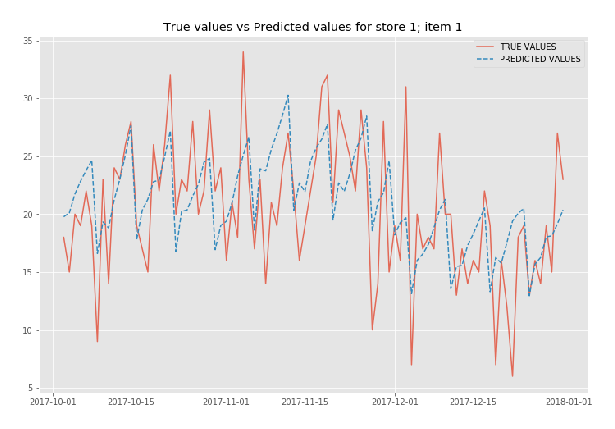
\includegraphics[width=.4\linewidth,height=.4\linewidth]{E:/tulip-flip/templatex-master/powerdot-tuliplab/logos/012.eps}
    \quad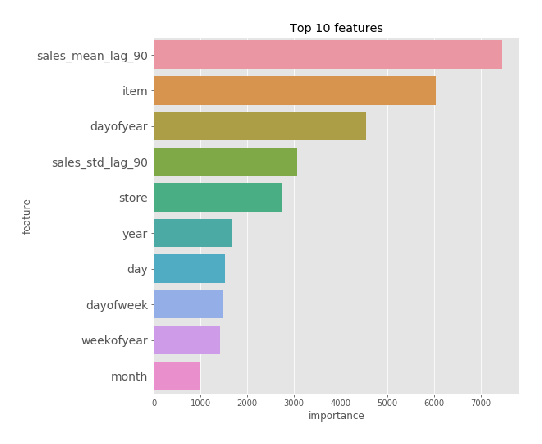
\includegraphics[width=.4\linewidth,height=.4\linewidth]{E:/tulip-flip/templatex-master/powerdot-tuliplab/logos/013.eps}
    \quad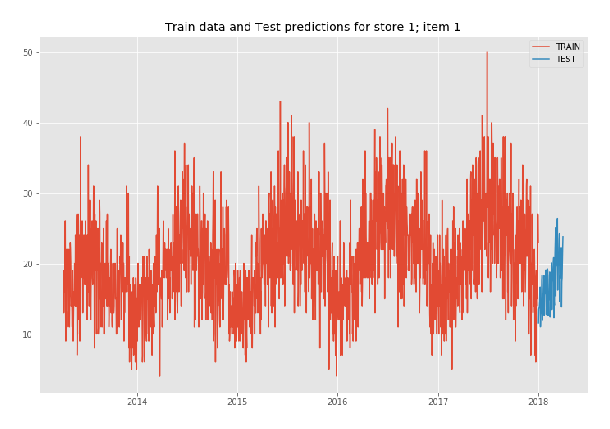
\includegraphics[width=.4\linewidth,height=.4\linewidth]{E:/tulip-flip/templatex-master/powerdot-tuliplab/logos/014.eps}	
  \end{center}
}
%%%%%%%%%% -------------------------------------------------------------------- %%%%%%%%%%


% Second column - second block
%%%%%%%%%% -------------------------------------------------------------------- %%%%%%%%%%
\block[titlewidthscale=1, bodywidthscale=1]
{Conclusion}
{
  \begin{description}
    \item[Data Analysis] Using visual methods to find connections and features within the dataset.
    \item[Feature Engineering] Find and extract important features. 
    \item[Modeling] Choose the suitable model parameters.
    \item[Prospcting] I woule like to select multiple models for comparison later.
  \end{description}
}
%%%%%%%%%% -------------------------------------------------------------------- %%%%%%%%%%


% Bottomblock
%%%%%%%%%% -------------------------------------------------------------------- %%%%%%%%%%
\colorlet{notebgcolor}{blue!20}
\colorlet{notefrcolor}{blue!20}
\note[targetoffsetx=8cm, targetoffsety=-4cm, angle=30, rotate=15,
radius=2cm, width=.26\textwidth]{
Acknowledgement
\begin{itemize}
    \item
    Thank you
 \end{itemize}
}

%\note[targetoffsetx=8cm, targetoffsety=-10cm,rotate=0,angle=180,radius=8cm,width=.46\textwidth,innersep=.1cm]{
%Acknowledgement
%}

%\block[titlewidthscale=0.9, bodywidthscale=0.9]
%{Acknowledgement}{
%}
%%%%%%%%%% -------------------------------------------------------------------- %%%%%%%%%%

\end{columns}


%%%%%%%%%% -------------------------------------------------------------------- %%%%%%%%%%
%[titleleft, titleoffsetx=2em, titleoffsety=1em, bodyoffsetx=2em,%
%roundedcorners=10, linewidth=0mm, titlewidthscale=0.7,%
%bodywidthscale=0.9, titlecenter]

%\colorlet{noteframecolor}{blue!20}
\colorlet{notebgcolor}{blue!20}
\colorlet{notefrcolor}{blue!20}
\note[targetoffsetx=-13cm, targetoffsety=-12cm,rotate=0,angle=180,radius=8cm,width=.96\textwidth,innersep=.4cm]
{
\begin{minipage}{0.3\linewidth}
\centering

\includegraphics[width=24cm]{logos/tulip-wordmark.eps}
\end{minipage}
\begin{minipage}{0.7\linewidth}
{ \centering
  FLIP00 FINAL PRESENTATION
  26/11/2019, Xi'an, China
}
\end{minipage}
}
%%%%%%%%%% -------------------------------------------------------------------- %%%%%%%%%%


\end{document}

%\endinput
%%
%% End of file `tikzposter-template.tex'.
